\documentclass[11pt]{amsart}
\usepackage{xcolor}
\usepackage{amsmath}
\usepackage{amssymb}
\usepackage{tikz}
\usepackage{pgfplots}
\pgfplotsset{compat=1.18}

\begin{document}

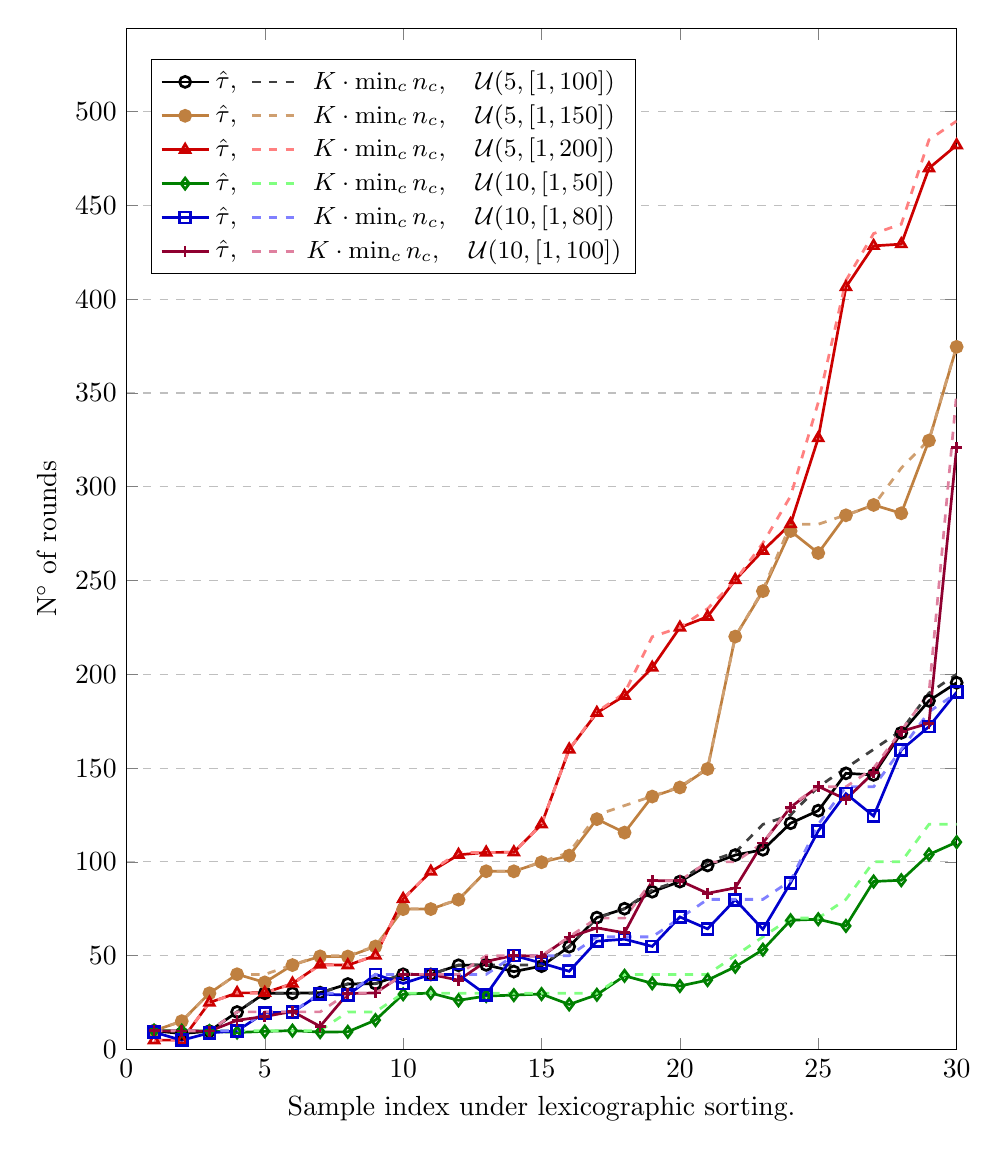
\begin{tikzpicture}
\begin{axis}[
every axis plot/.append style={line width=0.975pt},
    title={},
    width=\linewidth,
    height=2*\axisdefaultheight,
    xlabel={Sample index under lexicographic sorting.},
    ylabel={N$^{\circ}$ of rounds },
    xmin=0,
    xmax=30,
    ymin=0,
    ymajorgrids=true,
    grid style=dashed,
    legend style={anchor=north, legend columns=2, font=\small
    },
    legend pos=north west,
]

\addplot[
    color=black,
    mark=o,
    ]
    coordinates{
    (1,9.934)(2,8.4393)(3,9.7213)(4,19.953)(5,29.9434)(6,29.9405)(7,30.2424)(8,34.8575)(9,35.0919)(10,40.0434)(11,39.9822)(12,44.87)(13,45.0767)(14,41.5046)(15,44.4105)(16,54.7736)(17,70.2762)(18,75.0147)(19,84.078)(20,89.4784)(21,98.0616)(22,103.6288)(23,106.4502)(24,120.5994)(25,127.3087)(26,147.2139)(27,146.3782)(28,168.7921)(29,185.8892)(30,195.5127)
    };
    \addlegendentry{$\hat{\tau},~$}

\addplot[
    color=black!75!white,
    mark='-',
    line width=1pt,
    dashed
    ]
    coordinates{
    (1,10)(2,10)(3,10)(4,20)(5,30)(6,30)(7,30)(8,35)(9,35)(10,40)(11,40)(12,45)(13,45)(14,45)(15,45)(16,55)(17,70)(18,75)(19,85)(20,90)(21,100)(22,105)(23,120)(24,125)(25,140)(26,150)(27,160)(28,170)(29,190)(30,200)
    };
    \addlegendentry{$K \cdot \min_c n_c, ~~~\mathcal{U}(5,[1,100])$}

\addplot[
    color=brown,
    mark=*,
    ]
    coordinates{
    (1,9.9419)(2,15.0631)(3,29.928)(4,40.0772)(5,35.7298)(6,44.9667)(7,49.6117)(8,49.53)(9,54.8963)(10,74.7897)(11,74.8293)(12,79.8677)(13,94.9931)(14,94.9597)(15,99.8048)(16,103.339)(17,122.7884)(18,115.6039)(19,134.8273)(20,139.6631)(21,149.54)(22,220.1196)(23,244.3535)(24,276.4216)(25,264.6609)(26,284.7899)(27,290.3078)(28,285.8643)(29,324.6416)(30,374.6063)
    };
    \addlegendentry{$\hat{\tau},~$}

\addplot[
    color=brown!75!white,
    mark='-',
    line width=1pt,
    dashed
    ]
    coordinates{
    (1,10)(2,15)(3,30)(4,40)(5,40)(6,45)(7,50)(8,50)(9,55)(10,75)(11,75)(12,80)(13,95)(14,95)(15,100)(16,105)(17,125)(18,130)(19,135)(20,140)(21,150)(22,220)(23,245)(24,280)(25,280)(26,285)(27,290)(28,310)(29,325)(30,375)
    };
    \addlegendentry{$K \cdot \min_c n_c, ~~~\mathcal{U}(5,[1,150])$}

\addplot[
    color=red!80!black,
    mark=triangle,
    ]
    coordinates{
    (1,4.9415)(2,4.9469)(3,24.9603)(4,30.1307)(5,30.1822)(6,35.1324)(7,45.2338)(8,44.9019)(9,50.0285)(10,80.246)(11,94.8009)(12,103.7654)(13,105.0236)(14,105.1129)(15,120.0322)(16,159.9623)(17,179.4645)(18,188.5762)(19,203.5655)(20,224.9599)(21,230.7413)(22,250.3201)(23,265.9379)(24,280.1344)(25,325.9412)(26,406.4677)(27,428.452)(28,429.3769)(29,469.8347)(30,482.1521)
    };
    \addlegendentry{$\hat{\tau},~$}

\addplot[
    color=red!50!white,
    mark='-',
    line width=1pt,
    dashed
    ]
    coordinates{
    (1,5)(2,5)(3,25)(4,30)(5,30)(6,35)(7,45)(8,45)(9,50)(10,80)(11,95)(12,105)(13,105)(14,105)(15,120)(16,160)(17,180)(18,190)(19,220)(20,225)(21,235)(22,250)(23,270)(24,295)(25,345)(26,410)(27,435)(28,440)(29,485)(30,495)
    };
    \addlegendentry{$K \cdot \min_c n_c, ~~~\mathcal{U}(5,[1,200])$}

\addplot[
    color=green!50!black,
    mark=diamond,
    ]
    coordinates{
    (1,10.037)(2,10.0036)(3,9.7693)(4,9.0274)(5,9.6171)(6,10.0195)(7,9.2534)(8,9.378)(9,15.63)(10,29.4404)(11,30.04)(12,26.1642)(13,28.4717)(14,28.9556)(15,29.5194)(16,23.9713)(17,29.1268)(18,39.2412)(19,35.2513)(20,33.8035)(21,36.949)(22,44.0554)(23,53.1577)(24,68.8683)(25,69.4012)(26,65.8378)(27,89.5372)(28,90.2103)(29,103.9039)(30,110.5215)
    };
    \addlegendentry{$\hat{\tau},~$}

\addplot[
    color=green!50!white,
    mark='-',
    line width=1pt,
    dashed
    ]
    coordinates{
    (1,10)(2,10)(3,10)(4,10)(5,10)(6,10)(7,10)(8,20)(9,20)(10,30)(11,30)(12,30)(13,30)(14,30)(15,30)(16,30)(17,30)(18,40)(19,40)(20,40)(21,40)(22,50)(23,60)(24,70)(25,70)(26,80)(27,100)(28,100)(29,120)(30,120)
    };
    \addlegendentry{$K \cdot \min_c n_c, ~~~\mathcal{U}(10,[1,50])$}

\addplot[
    color=blue!80!black, %red!85!white,
    mark=square,
    ]
    coordinates{
    (1,9.1749)(2,4.879)(3,8.7873)(4,9.9205)(5,19.5763)(6,19.8129)(7,29.5284)(8,28.9249)(9,39.9907)(10,35.169)(11,39.9602)(12,39.9108)(13,29.141)(14,50.0785)(15,46.0334)(16,41.647)(17,57.6858)(18,58.7554)(19,54.9278)(20,70.6439)(21,64.2634)(22,79.8152)(23,64.0309)(24,88.8161)(25,116.4721)(26,136.3903)(27,124.4048)(28,159.6326)(29,172.1167)(30,190.4695)
    };
    \addlegendentry{$\hat{\tau},~$}

\addplot[
    color=blue!50!white,
    mark='-',
    line width=1pt,
    dashed
    ]
    coordinates{
    (1,10)(2,10)(3,10)(4,10)(5,20)(6,20)(7,30)(8,30)(9,40)(10,40)(11,40)(12,40)(13,40)(14,50)(15,50)(16,50)(17,60)(18,60)(19,60)(20,70)(21,80)(22,80)(23,80)(24,90)(25,120)(26,140)(27,140)(28,160)(29,180)(30,190)
    };
    \addlegendentry{$K \cdot \min_c n_c, ~~~\mathcal{U}(10,[1,80])$}

\addplot[
    color=purple!75!black,
    mark=+,
    ]
    coordinates{
    (1,9.9158)(2,9.8035)(3,9.736)(4,15.5321)(5,17.5608)(6,20.2144)(7,12.2969)(8,29.7609)(9,30.1136)(10,39.9526)(11,39.9962)(12,36.9035)(13,46.9319)(14,50.0927)(15,49.6191)(16,59.8711)(17,64.7855)(18,62.1687)(19,89.9929)(20,89.9396)(21,83.2425)(22,86.095)(23,110.1173)(24,129.1453)(25,140.2527)(26,133.337)(27,147.6135)(28,169.586)(29,173.9076)(30,320.8101)
    };
    \addlegendentry{$\hat{\tau},~$}

\addplot[
    color=purple!50!white,
    mark='-',
    dashed
    ]
    coordinates{
    (1,10)(2,10)(3,10)(4,20)(5,20)(6,20)(7,20)(8,30)(9,30)(10,40)(11,40)(12,40)(13,50)(14,50)(15,50)(16,60)(17,70)(18,70)(19,90)(20,90)(21,100)(22,100)(23,110)(24,130)(25,140)(26,140)(27,150)(28,170)(29,190)(30,350)
    };
    \addlegendentry{$K \cdot \min_c n_c, ~~~\mathcal{U}(10,[1,100])$}

\end{axis}


\end{tikzpicture}

\end{document}